\chapter{Solving Linear Equations}

\subsection*{Section~\protect{\ref{S:2.1}} Systems of Linear Equations and
Matrices}
\rhead{S:2.1}{SYSTEMS OF LINEAR EQUATIONS AND MATRICES}

\exer{c2.1.8a} $(x,y) = (2,4)$.

\exer{c2.1.8b} $(x,y,z) = (-\frac{2}{3}, -1, 3)$.

\exer{c2.1.8c} $(x,y) = (-4,1)$.

\exer{c2.1.8A} The matrices for the three systems are,
\[
\mattwo{2}{-1}{3}{0}, \quad
\matthree{3}{-4}{0}{0}{2}{1}{0}{0}{3}, \AND
\mattwo{-2}{1}{3}{3}.
\]

\exer{c2.1.9}
\ans The system in part (a) has an infinite number of solutions, whereas
the system in part (b) has no solution.

\soln (a) Replace $x$ in the second and third equations with
$4 + y$ to obtain $4y - 2z = -10$ and $6y - 3z = -15$.  Since these
equations have identical solutions, the system can be restated as
\[
\begin{array}{rrrrrrr}
x & = & y & + & 4 \\ 
z & = & -2y & + & 5\end{array}
\]
So, for each choice of $y$, there exists a single solution.  For
example, if $y = 1$, then $x = 5$ and $z = 3$; or if $y = 0$, then
$x = 4$ and $z = 5$.

(b) If we again substitute for $x$ using the first equation, the
second and third equations become
\[
2y - 3z = -2 \AND 2y - 3z = -4
\]

These two expressions contradict each other, so there is no solution
for this system.

\newpage
\exer{c2.1.10}
Dick is 17 and Jane is 9.


\exer{c2.1.11}
(a) \ans The quadratic $p(x) = -x^2 + 5x + 1$ satisfies these conditions.

\soln Since $p(x) = ax^2 + bx + c$ for any quadratic equation, we find
this solution by evaluating $p(0) = 1$, $p(1) = 5$, and $p(-1) = -5$,
which yields the system of equations
\[
\begin{array}{lrrrrrrrr}
p(0) & = & & & & & c & = & 1 \\
p(1) & = & a & + & b & + & c & = & 5 \\
p(-1) & = & a & - & b & + & c & = & -5\end{array}
\]
We solve this system to obtain $(a,b,c) = (-1,5,1)$, then substitute
these coefficients into the general quadratic.

(b) Let $p(x) = ax^2 + bx + c$ be a quadratic equation.  Then, the
assumptions $p(0) = L$, $p(1) = M$, and $p(-1) = N$ imply:
\[
\begin{array}{lrrrrrrrr}
p(0) & = & & & & & c & = & L \\
p(1) & = & a & + & b & + & c & = & M \\
p(-1) & = & a & - & b & + & c & = & N\end{array}
\]
The unique solution to this system is $(a,b,c) =
(\frac{M + N - 2L}{2},\frac{M - N}{2},L)$.

(c) Substituting $q(x_i) = A_i$, for $i = 1,2,3$, into the standard
quadratic equation $q(x) = ax^2 + bx + c$ yields
\[
\begin{array}{ccccccc}
ax_1^2 & + & bx_1 & + & c & = & A_1 \\
ax_2^2 & + & bx_2 & + & c & = & A_2 \\
ax_3^2 & + & bx_3 & + & c & = & A_3\end{array}
\]
Finding the appropriate quadratic polynomial would be equivalent to
solving this system of linear equations for $a$, $b$, and $c$ in
terms of $A_1$, $A_2$, and $A_3$.




\exer{c2.1.1}
Type {\tt A}$\backslash${\tt b}, to get
\begin{verbatim}
ans =
    0.7060
    2.4963
   -2.9778
   -1.7627
   -0.1163
    0.2654
\end{verbatim}

\exer{c2.1.2} Type {\tt A(2,1) = -5}.  \Matlab responds with
\begin{verbatim}
A =
    -1     1     2
    -5     1     2
\end{verbatim}

\newpage
\exer{c2.1.3} Type {\tt b(3) = 13} to obtain
\begin{verbatim}
b =
     1
     2
    13
\end{verbatim}

\exer{c2.1.4} \ans According to \Matlabp,
\begin{verbatim}
ans =
  -12.0495
   -0.8889
    7.8384
\end{verbatim}
\soln Write the system as $Ax = b$, where:
\begin{verbatim}
A =                                             b = 
    2.0000   -4.5000    3.1000                     4.2000
    1.0000    1.0000    1.0000                    -5.1000
    1.0000   -6.2000    1.0000                     1.3000
\end{verbatim}
then type {\tt A}$\backslash${\tt b} to solve.

\exer{c2.1.5}
{\tt A}$\backslash${\tt b} is not defined when $A(2,2) = -1$.

\exer{c2.1.6} Computer experiment.

\exer{c2.1.7} \ans The vector of solutions is:
\begin{verbatim}
ans =
    7.3828
    4.1016
    4.5313
   10.6250
\end{verbatim}
\soln First, translate the data in the table to a system of linear
equations, relating the quantities of $S_1$, $S_2$, $S_3$, and $S_4$
in the mixture to the quantities of vitamins $A$, $B$, $C$, and $F$. 
The first equation is $.25S_1 + .19S_2 + .20S_3 + .03S_4 = A$, and
the other three equations correspond to the other vitamins.  From
this data, find the coefficient matrix $A$ for the system.  The desired
quantities of each vitamin form the solution vector $b$.
\begin{verbatim}
A =                                             b =
    0.2500    0.1900    0.2000    0.0300           3.8500
    0.0200    0.1400    0.0200    0.1400           2.3000
    0.0800    0.0400    0.0100         0           0.8000
    0.2500    0.3100    0.2500    0.1600           5.9500
\end{verbatim}
As in the previous problems, the system can be solved by
typing {\tt A}$\backslash${\tt b}.

\para If $b(2) = 2.00$ instead of $2.30$, then
{\tt A}$\backslash${\tt b} yields

\begin{verbatim}
ans =
   22.4023
  -27.8320
   12.1094
   37.1875
\end{verbatim}
Note that the components of the answer vector refer to weights of
substances, which cannot be negative.  This answer contains a negative
component; so although a mathematically valid solution exists, we
cannot mix the substances in such a way that

$b = \left(\begin{array}{r} 3.85 \\ 2.00 \\ 0.80 \\ 5.95\end{array} \right)$.



\subsection*{Section~\protect{\ref{S:2.2}} The Geometry of Low-Dimensional
Solutions}
\rhead{S:2.2}{THE GEOMETRY OF LOW-DIMENSIONAL SOLUTIONS}

\exer{c2.2.5}
\ans The equation of the desired plane is $2x + 3y + z = -5$.

\soln Note that a vector perpendicular to a plane is orthogonal
to any vector connecting two points in the plane.  So,
if $X_0 = (-1,-2,3)$ is one point in the plane perpendicular to
$N = (2,3,1)$ and $X = (x,y,z)$ is any other point in that plane,
then $(X - X_0) \cdot N = 0$.  Substituting into this formula, we obtain
\[
2(x + 1) + 3(y + 1) + 1(z - 3) = 0\quad\mbox{or}\quad
2x + 3y + z = -5.
\]

\exer{c2.2.6}
Examples:

$\left. \begin{array}{rrrrr}
x & + & y & = & 2 \\
x & - & y & = & 0\end{array} \right\}$
unique solution

$\left. \begin{array}{rrrrr}
x & + & y & = & 2 \\
2x & + & 2y & = & 4\end{array} \right\}$
infinite number of solutions

$\left. \begin{array}{rrrrr}
x & + & y & = & 2 \\
x & + & y & = & 4\end{array} \right\}$
no solutions

\exer{c2.2.7}
\ans The equation for the plane is $z = x$.

\soln Note that the plane goes through the origin and contains the
vectors $(1,0,1)$ and $(2,-1,2)$, and therefore contains the points
$(0,0,0)$, $(1,0,1)$, and $(2,-1,2)$.  The general equation for a plane
is $ax + by + cz = d$.  We can substitute the coordinates of the three
points into this equation to get the linear system
\[
\begin{array}{rrrrrrr}
 & & & & 0 & = & d \\
a & & & + & c & = & d \\
2a & - & b & + & 2c & = & d\end{array}
\]
We can solve the system by substitution to get $b = d = 0$ and $a = -c$,
which yields the equation of the plane.

\exer{c2.2.8}
\ans One such system is:
\[
\begin{array}{rrrrrrr}
x & - & y & + & z & = & 0 \\
2x & + & y & - & 4z & = & 0\end{array}
\]
\soln The solution set contains all multiples of the vector $(1,2,1)$,
so it contains the origin, since $0(1,2,1) = (0,0,0)$.  The equation
of any plane containing the origin is $ax + by + cz = 0$. 
Substituting the point $(1,2,1)$ implies that $a + 2b + c = 0$. 
Any two equations which satisfy that condition and are not multiples
of one another will have the appropriate line as a solution set. 
For example, let $(a,b,c) = (1,-1,1)$ in the first equation, and
$(a,b,c) = (2,1,-4)$ in the second equation to obtain the system
given here.



\exer{c2.2.9}
(a) $u = (2,2,1)$, since we know that the normal vector to the plane
$ax + by + cz = d$ is $(a,b,c)$.

(b) $v = (1,1,2)$.

(c) $\cos\theta = \frac{u \cdot v}{||u||\;||v||} = \frac{2}{\sqrt{6}}$.
In \Matlabp, type {\tt acos(2/sqrt(6))*180/pi} to obtain $\theta =
35.2644^\circ$.

\exer{c2.2.10}
The system has no solutions because there is no point at which the three
planes intersect.  Figure~\ref{c2.2.10}a shows the \Matlab graph of
the system.  The commands {\tt view([0 -1 0])} and 
{\tt axis([-7 3 -3 3 -1 3])}
produce a view of the graph in which the geometry
can be seen, shown in Figure~\ref{c2.2.10}b.
Since there is no $y$ term in any of the equations, all three planes
are perpendicular to this view, and therefore appear as lines in the
graph.

\begin{figure}[htb]
                       \centerline{%
                       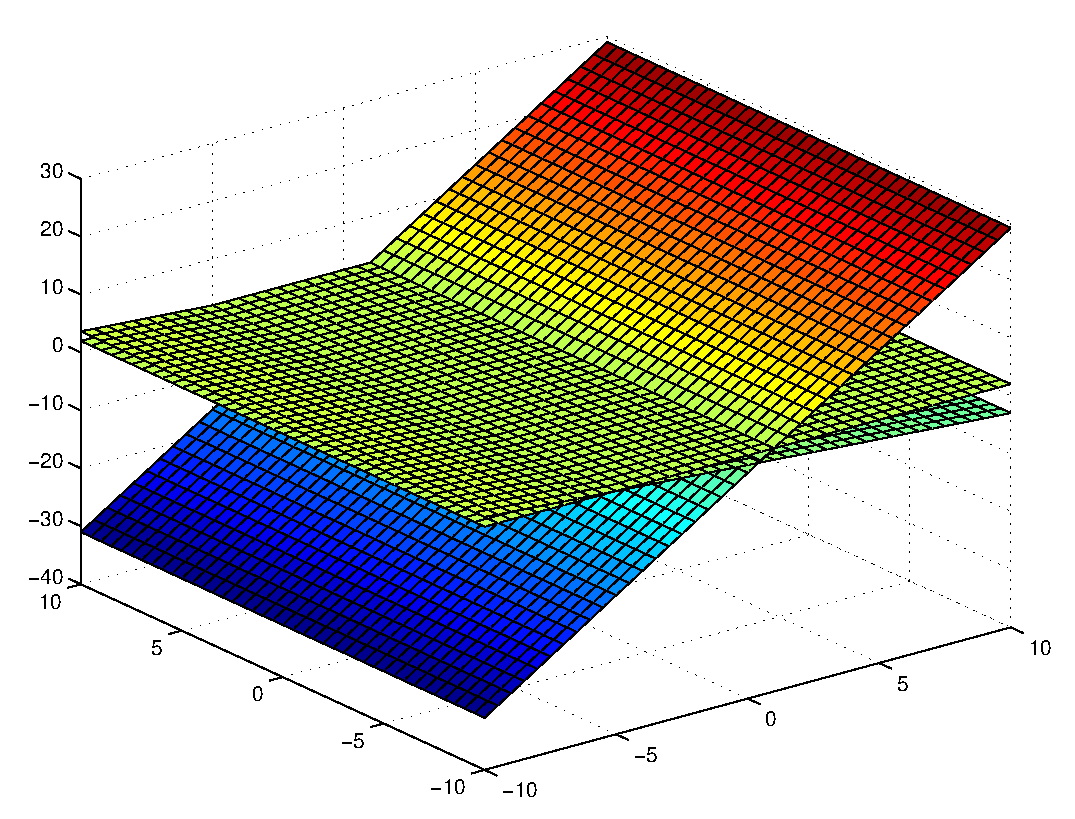
\psfig{file=exfigure/2-2-10a.eps,width=2.75in}
                       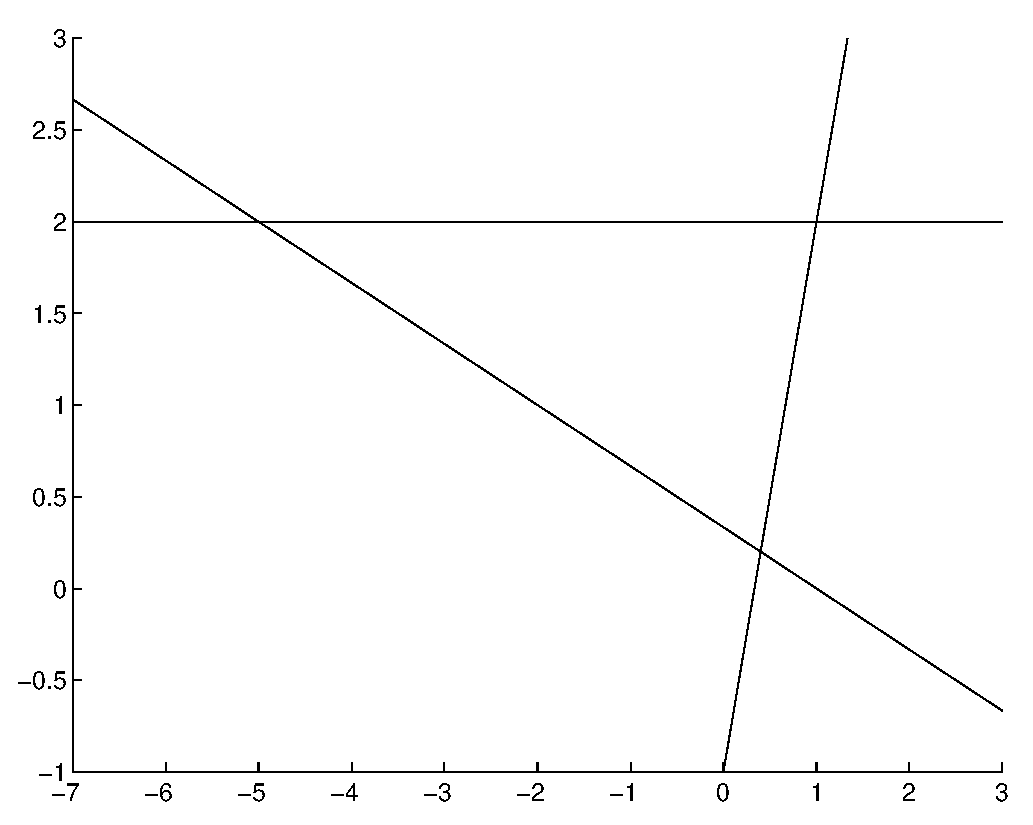
\psfig{file=exfigure/2-2-10b.eps,width=2.75in}}
		\exercaptwo{c2.2.10}
\end{figure}





\exer{c2.2.1}
\ans $(x,y) \approx (2.15,-1.54)$.

\soln In \Matlab, graph the system by typing:
\begin{verbatim}
x = linspace(-5,5,100);
y = -1 - x/4;
plot(x,y)
xlabel('x')
ylabel('y')
hold on
y = 4/3 - 4*x/3;
plot(x,y)
axis('equal')
grid
\end{verbatim}

Using the {\tt zoom} command, we can zoom in on the graph of
Figure~\ref{c2.2.1} until the intersection of the lines is
visible at an accuracy of two decimal places.  

\begin{figure}[htb]
                       \centerline{%
                       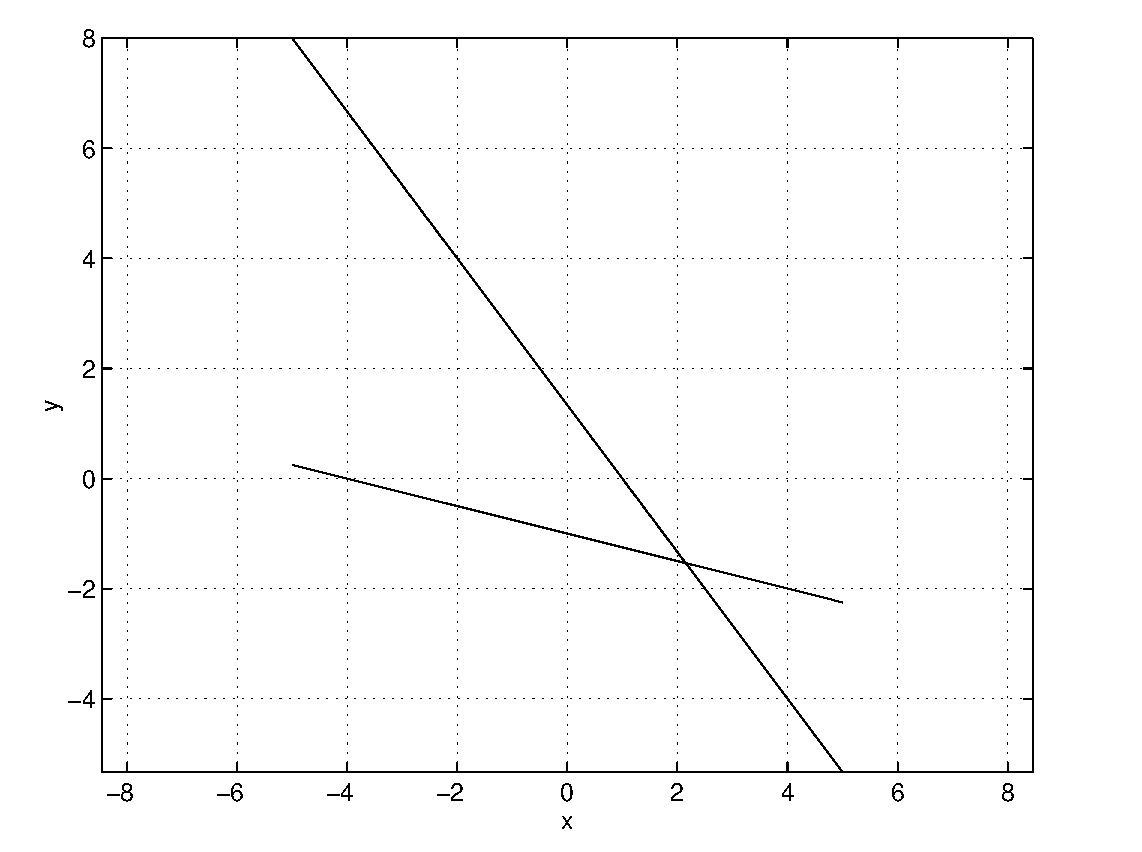
\psfig{file=exfigure/2-2-1a.eps,width=2.75in}
                       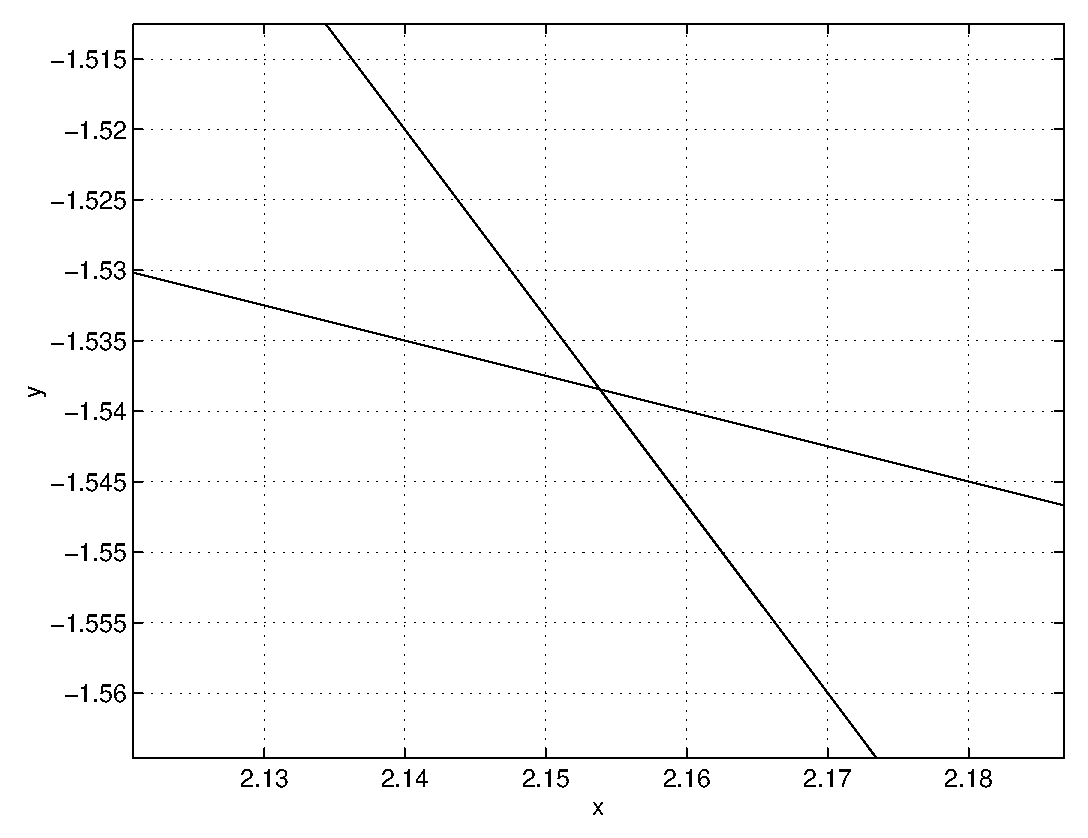
\psfig{file=exfigure/2-2-1b.eps,width=2.75in}}
		\exercaptwo{c2.2.1}
\end{figure}

\exer{c2.2.2}
$(x,y) \approx (-0.26,-0.73)$.

\newpage
\exer{c2.2.3}
\ans $(x,y,z) = (1,3,-1)$.

\soln The commands to instruct \Matlab to graph this three dimensional
system are:
\begin{verbatim}
[x,y] = meshgrid(-10:0.5:10);
z = (-11 - 3*x + 4*y)/2;
surf(x,y,z)
hold on 
z = 7 - 2*x - 2*y;
surf(x,y,z)
hold on
z = (7 + x - y)/(-5);
surf(x,y,z)
\end{verbatim}
It is hard to determine a solution for the system from this graph.
The command {\tt axis([xmin xmax ymin ymax zmin zmax])} can make the
graph clearer by zooming in on a specific range of points, but a
numerically accurate solution is difficult to obtain graphically in
three dimensions.  Obtain an accurate solution using the command
{\tt A}$\backslash${\tt b} in \Matlabp.

\exer{c2.2.4}
\ans The solution set is a line because the three planes intersect in a line.

\soln If the left-hand side of the system is entered into \Matlab as
matrix {\tt A}, and the solution vector is entered as {\tt b}, then
typing {\tt A}$\backslash${\tt b} yields
\begin{verbatim}
Warning: Matrix is singular to working precision.
ans =
   Inf
   Inf
   Inf
\end{verbatim}

\exer{c2.2.a5}
\ans The function has three relative maxima on this interval.

\soln Graph the function in \Matlab using the commands:
\begin{verbatim}
x = linspace(-2,3);
y = 2 - x.*sin(x.^2 - 1);
plot(x,y)
\end{verbatim}
Determine the number of relative maxima numerically from the graph, which
is shown in Figure~\ref{c2.2.a5}.

\begin{figure}[htb]
                       \centerline{%
                       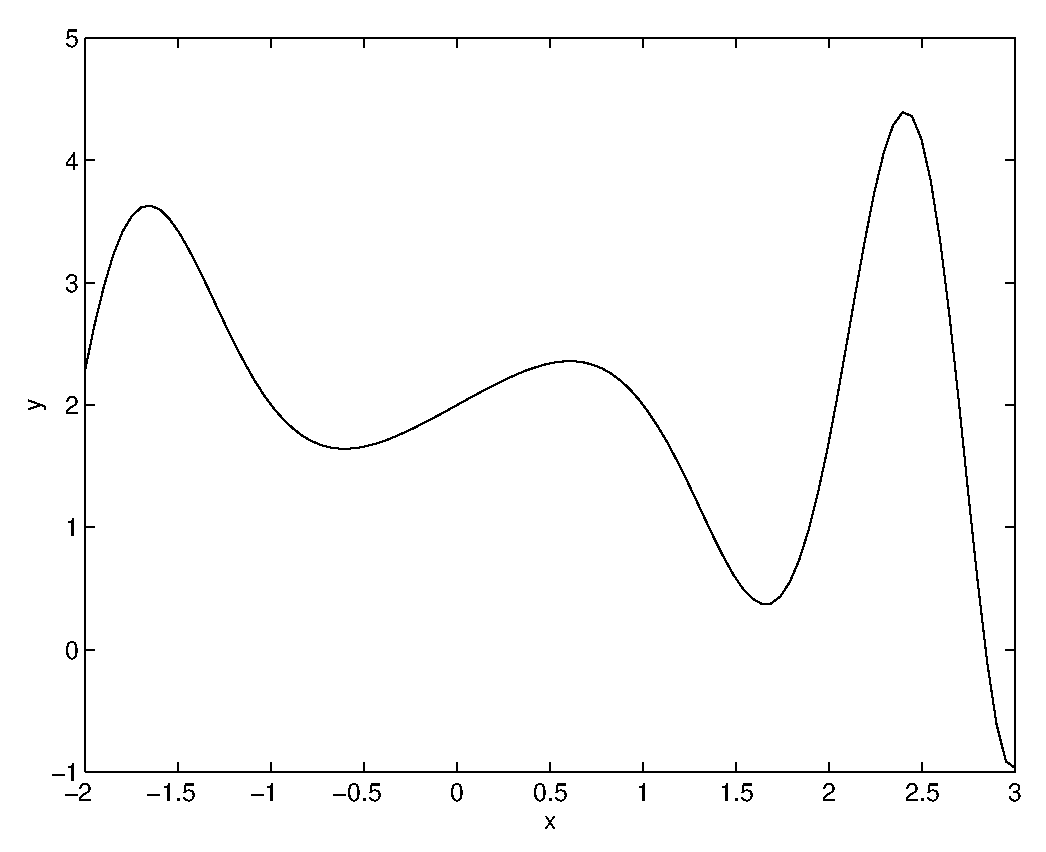
\psfig{file=exfigure/2-2-a5.eps,width=3.0in}}
		\exercap{c2.2.a5}
\end{figure}






\subsection*{Section~\protect{\ref{S:Gauss}} Gaussian Elimination}
\rhead{S:Gauss}{GAUSSIAN ELIMINATION}


\exer{c2.3.6a} The matrix is not in reduced echelon form.

\newpage
\exer{c2.3.6b} The matrix is in reduced echelon form.

\exer{c2.3.6c} The matrix is not in reduced echelon form.

\exer{c2.3.7a} The $1^{st}$ and $3^{rd}$ columns of the matrix contain
pivots.  The solutions of the system are:

\[
\left(\begin{array}{r} x_1 \\ x_2 \\ x_3\end{array} \right)
= \left(\begin{array}{c} -4x_2 \\ x_2 \\ 5\end{array} \right)
\]

\exer{c2.3.7b} The $1^{st}$, $3^{rd}$, and $5^{th}$ columns of the matrix
contain pivots.  Since the last row of the matrix translates to the linear
equation $0 = 1$, the system is inconsistent, and there are no solutions.

\exer{c2.3.7c} The $1^{st}$ and $3^{rd}$ columns of the matrix contain
pivots.  The solutions of the system are:

\[
\left(\begin{array}{r} x_1 \\ x_2 \\ x_3\\ x_4\end{array} \right)
= \left(\begin{array}{c} 1 + 6x_2 \\ x_2 \\ 9 \\ x_4\end{array} \right)
\]

\exer{c2.3.8}
(a)
Two matrices are row equivalent if there is a sequence of row operations
that leads from one to the other.  In this case:

1. Divide the $1^{st}$ row of \Ref{e:2x2} by $a$.

2. Subtract $c$ times the $1^{st}$ row from the $2^{nd}$ row.

The result is
\[
\left(\begin{array}{cc} 1 & \frac{b}{a} \\ 0 & \frac{a - bc}{a}\end{array}
\right).
\]

(b) If $a \neq bc$, then we can row reduce \Ref{e:2x2} to $I_2$ by
performing the two row operations in part (a), followed by:

3. Multiply the $2^{nd}$ row by $\frac{a}{a - bc}$.

4. Subtract $\frac{b}{a}$ times the second row from the first row.

This will give us the identity matrix $I_2$.

\para If $a = bc$, then $\frac{a - bc}{a} = 0$, and the matrix is
\[
\left(\begin{array}{cc} 1 & \frac{b}{a} \\ 0 & 0\end{array} \right).
\]
which has only one pivot and cannot be row reduced to $I_2$.

\exer{c2.3.9}
\ans The solution to this system is
\[
\left(\begin{array}{c} x_1 \\ x_2 \\ x_3\end{array}\right) =
\left(\begin{array}{c} 0 \\ x_3 - 1 \\ x_3\end{array}\right),
\]
where $x_3$ is any real number.

\soln Row reduce the augmented matrix of the system:
\[
\left(\begin{array}{rrr|r} 1 & -1 & 1 & 1 \\ 2 & 1 & -1 & -1\end{array}\right)
\longrightarrow
\left(\begin{array}{rrr|r} 1 & 0 & 0 & 0 \\ 0 & 1 & -1 & -1\end{array}\right).
\]
Although $(1,2,2)$ is not a solution to this system, there is a solution
for which $x_3 = 2$, namely $(0,1,2)$.

\exer{c2.3.10a} The augmented matrix for this system is
\[
\left(\begin{array}{rrr|r} 1 & -1 & 1 & 1 \\ 4 & 1 & 1 & 5 \\
2 & 3 & -1 & 2\end{array}\right)
\]
We can row reduce this matrix to reduced echelon form, obtaining
\[
\left(\begin{array}{rrr|r} 1 & 0 & \frac{2}{5} & \frac{6}{5} \\
0 & 1 & -\frac{3}{5} & \frac{1}{5} \\ 0 & 0 & 0 & 1\end{array}\right)
\]
The last row of the reduced system implies that $0 = 1$, so the system
is inconsistent and has no solutions.

\exer{c2.3.10b} The augmented matrix for this system is
\[
\left(\begin{array}{rrrr|r} 2 & -1 & 1 & 1 & 1 \\ 1 & 2 & -1 & 1 & 7
\end{array}\right)
\]
which can be row reduced to
\[
\left(\begin{array}{rrrr|r} 1 & 0 & \frac{1}{5} & \frac{3}{5} &
\frac{9}{5} \\ 0 & 1 & -\frac{3}{5} & \frac{1}{5} & \frac{13}{5}
\end{array}\right).
\]
The solution set is therefore
\[
\left(\begin{array}{c} x_1 \\ x_2 \\ x_3 \\ x_4\end{array}\right) =
\left(\begin{array}{c} \frac{9}{5} - \frac{1}{5}x_3 - \frac{3}{5}x_4
\\ \frac{13}{5} + \frac{3}{5}x_3 - \frac{1}{5}x_4 \\ x_3 \\ x_4
\end{array}\right).
\]

\exer{c2.3.11a}
\ans (a) The system has infinitely many solutions.

(b) One variable can be assigned arbitrary values.

\soln The row-reduced form of the matrix is:

\[
\left(\begin{array}{rrr|r} 1 & 0 & 0 & 3 \\ 0 & 1 &
\frac{1}{2} & \frac{1}{2} \\ 0 & 0 & 0 & 0\end{array}\right).
\]

\exer{c2.3.11b}
\ans The system has no solutions.

\soln The row-reduced form of the matrix is:
\[
\left(\begin{array}{rrrr|r} 1 & 2 & 0 & 0 & 3 \\
0 & 1 & 1 & 0 & 1 \\ 0 & 0 & 0 & 0 & 1\end{array}\right).
\]

\exer{c2.3.11c}
\ans The system has a unique solution.

\soln The row-reduced form of the matrix is:
\[
\left(\begin{array}{rrr|r} 1 & 0 & 2 & 1 \\ 0 & 1 & 0 & \frac{2}{5}
\\ 0 & 0 & 1 & \frac{3}{4}\end{array}\right).
\]

\exer{c2.3.11d}
\ans (a) The system has infinitely many solutions.

(b) Two variables can be assigned arbitrary values.

\soln The row-reduced form of the matrix is:
\[
\left(\begin{array}{rrrr|r} 1 & 0 & 2 & 0 & 3 \\ 0 & 1 & \frac{2}{3}
& \frac{1}{3} & \frac{10}{3} \\ 0 & 0 & 0 & 0 & 0 \\ 0 & 0 & 0 & 0 & 0
\end{array}\right).
\]

\newpage
\exer{c2.3.12a} \ans The system is linear.

\exer{c2.3.12b} \ans The system is linear.

\exer{c2.3.12c} \ans The system is not linear.

\soln The term $3x_1x_2$ contains two variables, and the term $x_2^2$
contains a variable squared.  Thus, these terms are not linear.

\exer{c2.3.12d} \ans The system is linear.

\exer{c2.3.12e} \ans The system is not linear.

\soln The term $\sin(x_2)$ is not linear.


\exer{c2.3.1a} \ans The row echelon form matrix is
\begin{verbatim}
A = 
    1.0000    0.5000    0.5000
         0         0    1.0000
\end{verbatim}
\soln Enter the augmented matrix into \Matlab as $A$, then reduce to
row echelon form by typing:
\begin{verbatim}
A(1,:) = A(1,:)/2
A(2,:) = A(2,:) - 4*A(1,:)
\end{verbatim}
The linear system that this matrix represents is inconsistent, since
the $2^{nd}$ row of the reduced matrix represents the equation $0 = 1$.

\exer{c2.3.1b} The row-reduced matrix is:
\begin{verbatim}
A =
    1.0000   -1.3333         0    0.6667
         0    1.0000    1.5000    0.5000
         0         0    1.0000   -0.1429
\end{verbatim}
This matrix represents a consistent linear system.

\exer{c2.3.1c} The row-reduced matrix is:
\begin{verbatim}
A =
    1.0000   -0.5000   -4.5000   -0.5000
         0    1.0000    2.1111    0.7778
         0         0         0    2.0000
\end{verbatim}
This matrix represents an inconsistent linear system.

\newpage
\exer{c2.3.2} The row echelon form is:
\begin{verbatim}
A = 
       0   1.0000   2.0000   1.0000  14.0000  21.0000        0  -1.0000
       0        0        0   1.0000   3.0000   5.0000        0   9.0000
       0        0        0        0   1.0000  -0.5000        0  -4.7143
       0        0        0        0        0   1.0000        0   0.3457
       0        0        0        0        0        0        0   1.0000
       0        0        0        0        0        0        0        0
\end{verbatim}


\exer{c2.3.3}
\ans The system's solution is
\[
\left(\begin{array}{c} x_1 \\ x_2 \\ x_3 \\ x_4\end{array}\right) =
\left(\begin{array}{c} -\frac{7}{4} - \frac{21}{8}x_4 \\ -\frac{9}{2} -
\frac{11}{4}x_4 \\ -\frac{19}{4} - \frac{25}{8}x_4 \\ x_4\end{array}\right)
\]
where $x_4$ is any real number.

\soln Note that the system of linear equations is related to the
augmented matrix
\begin{verbatim}
A = 
    2        3       -4        1        2
    3       -1       -1        2        4
    1       -7        5       -1        6
\end{verbatim}
which row reduces to
\begin{verbatim}
A =
    1       3/2      -2       1/2       1
    0        1     -10/11    -1/11    -2/11
    0        0        1      25/8    -19/4
\end{verbatim}
The system can then be solved by back substitution.

\exer{c2.3.4}
(a)
\begin{verbatim}
A =
   1.0000e+00   3.0000e+00   4.0000e+00
            0   1.0000e+00   1.4000e+00
            0            0            0
\end{verbatim}

(b)
$B = \left(\begin{array}{rrr}
1 & \frac{1}{3} & \frac{4}{3} \\
0 & 1 & -\frac{1}{5} \\
0 & 0 & 0\end{array} \right)$

(c)
\begin{verbatim}
B =
   1.0000e+00   3.3333e-01   1.3333e+00
            0   1.0000e+00  -2.0000e-01
            0            0   2.2204e-16
\end{verbatim}


(d) Note that switching the first two columns of matrix {\tt A} produces
matrix {\tt B}.  Suppose that {\tt A} and {\tt B} represent the left-hand
sides of linear systems with the same vector representing the right-hand
sides.  If the solution of system {\tt A} is $(x,y,z) = (a,b,c)$, then the
solution of system {\tt B} should be $(x,y,z) = (b,a,c)$.  However,
according to the row reduced matrices produced by \Matlab, the system
corresponding to {\tt B} has a unique solution, and the system
corresponding to {\tt A} does not.  Row reducing {\tt B} by hand shows
that there is not a unique solution.  \Matlab calculations provide one because of 
roundoff error.  The division by 3 in the first step of the row reduction
for {\tt B} causes a rounding inaccuracy.  Because of this, \Matlab
eventually computes a very small nonzero value for {\tt B}$(3,3)$
rather than the correct answer of 0.

\exer{c2.3.5}
\ans The polynomial $p(x) = -\frac{3}{44}x^3 + \frac{5}{11}x^2 +
\frac{5}{44}x + \frac{3}{2}$ satisfies the given conditions.

\soln Let $p(x) = ax^3 + bx^2 + cx + d$ be the general cubic polynomial. 
Then $p'(x) = 3ax^2 + 2bx + c$.  We can write the conditions on $p$ as a
system of linear equations:
\[
\begin{array}{rrrrrrrrr}
a & + & b & + & c & + & d & = & 2 \\
8a & + & 4b & + & 2c & + & d & = & 3 \\
3a & - & 2b & + & c & & & = & -1 \\
27a & + & 6b & + & c & & & = & 1\end{array}
\]
Using \Matlab, we solve for $a$, $b$, $c$, and $d$, obtaining the
vector of coefficients:
\begin{verbatim}
ans =
    -3/44
     5/11
     5/44
     3/2
\end{verbatim}





\subsection*{Section~\protect{\ref{S:2.4}} Reduction to Echelon Form}
\rhead{S:2.4}{REDUCTION TO ECHELON FORM}

\exer{c2.4.1}
The reduced echelon form of the matrix is:
\[
A = \left(\begin{array}{rrrr} 1 & 2 & 0 & 4 \\ 0 & 0 & 1 & 2 \\ 0 & 0 & 0
& 0\end{array}\right)
\]
The rank of $A$ is two, since the reduced echelon matrix has two nonzero
rows.

\exer{c2.4.1b}
The reduced echelon form of the matrix is:
\[
B=\left(\begin{array}{rrr} 1 & 0 & \frac{10}{3} \\ 
0 & 1 & \frac{1}{6} \\ 0 & 0 & 0 \end{array}\right)
\]
The rank of $B$ is two, since the reduced echelon matrix has two nonzero
rows.

\exer{c2.4.2}
\ans Four parameters are needed to specify all solutions.

\soln According to Theorem \ref{number}, $n - \ell$
parameters are needed to parameterize the set of all solutions of a
linear system, where $n$ is the number of unknowns, and $\ell$ is the
rank of the reduced echelon matrix.  In this case, $n = 7$ and $\ell =
3$.

\exer{c2.4.2b}
\ans Seven parameters are needed to specify all solutions.

\soln According to Theorem \ref{number}, $n - \ell$
parameters are needed to parameterize the set of all solutions of a
linear system, where $n$ is the number of unknowns, and $\ell$ is the
rank of the reduced echelon matrix.  In this case, $n = 12$ and $\ell =
5$.


\exer{c2.4.3a}
\ans Matrix $A$ is consistent and requires 3 parameters to enumerate
all solutions.

\soln
\begin{verbatim}
rref(A) = 
    1.0000         0    1.9474   -1.4211    2.2632    0.5789
         0    1.0000   -0.8947    0.8421   -0.5263   -0.1579
         0         0         0         0         0         0
         0         0         0         0         0         0
\end{verbatim}

\exer{c2.4.3b}
\ans Matrix $B$ is consistent and requires 1 parameter.

\soln
\begin{verbatim}
rref(B) =
    1.0000    2.0000         0         0    1.0556
         0         0    1.0000         0   -0.2222
         0         0         0    1.0000   -0.1111
\end{verbatim}

\exer{c2.4.3c}
\ans Matrix $C$ is inconsistent.

\soln
\begin{verbatim}
rref(C) =
     1     0    -5     0
     0     1     3     0
     0     0     0     1
\end{verbatim}

\newpage
\exer{c2.4.3d}
\ans Matrix $D$ is consistent and requires 2 parameters.

\soln
\begin{verbatim}
rref(D) =
    1.0000    2.0261         0    0.9174   -0.3047
         0         0    1.0000         0    1.0827
         0         0         0         0         0
         0         0         0         0         0
\end{verbatim}

\exer{c2.4.4a} \ans The rank of the matrix is $1$.

\soln Use the \Matlab command {\tt rank(A)} to determine the rank of a 
matrix $A$.

\exer{c2.4.4b} The rank of the matrix is $3$.

\exer{c2.4.4c} The rank of the matrix is $2$.


\subsection*{Section~\protect{\ref{S:specialcoeff}} Linear Equations with
Special Coefficients}
\rhead{S:specialcoeff}{LINEAR EQUATIONS WITH SPECIAL COEFFICIENTS}

\exer{c2.5.1}
$\left(\begin{array}{c} x_1 \\ x_2\end{array}\right) =
\left(\begin{array}{r} \frac{3}{2} - \frac{1}{2}i \\ -\frac{1}{2} -
\frac{1}{2}i\end{array}\right).$

\exer{c2.5.1A}
$\left(\begin{array}{c} x_1 \\ x_2 \\ x_3\end{array}\right) =
\left(\begin{array}{r} 
\frac{43}{24} \\ -\frac{1}{8} \\ \frac{1}{3} \end{array}\right)$.

\exer{c2.5.1B}
$\left(\begin{array}{c} x_1 \\ x_2\end{array}\right) =
\left(\begin{array}{r} \frac{1}{2} \\ -\frac{1}{2} \end{array}\right)$.


\exer{c2.5.2a}
Enter the left-hand side of each system as matrix {\tt A} 
and the right-hand side as vector {\tt b}:

\begin{verbatim}
A =                           
    0.1000    2.2361   -2.0000
   -1.7321    3.1416   -2.6000
    1.0000   -7.0000    1.5708

b =                              A\b =
   1.0000                          -7.2216
  14.3000                          -1.9048
   1.4142                          -2.9907
\end{verbatim}

\exer{c2.5.2b}
Enter the left-hand side of each system as matrix {\tt A} 
and the right-hand side as vector {\tt b}:

\begin{verbatim}
A =
   4.0000 - 1.0000i    2.0000 + 3.0000i
        0 + 1.0000i   -4.0000          

b =                              A\b =
        0 - 1.0000i                 0.3006+ 0.2462i
   2.2000                          -0.6116+ 0.0751i
\end{verbatim}

\exer{c2.5.2c}
Enter the left-hand side of each system as matrix {\tt A} 
and the right-hand side as vector {\tt b}

\begin{verbatim}
A =
   2.0000 + 1.0000i    1.4142 - 3.0000i  -10.6600
  14.0000                   0 - 2.2361i   10.2000 - 1.0000i
  -4.2760              2.0000             -4.0000 + 2.0000i

b =                              A\b =
   4.2300                           0.2060- 0.1139i
   3.0000 - 1.6000i                 0.1982+ 0.6586i
        0 + 1.4142i                -0.1358+ 0.0296i
\end{verbatim}





















